\documentclass[a4paper, 12pt]{book}
\usepackage[a4paper, left=2.5cm, right=2.5cm, top=3cm, bottom=3cm]{geometry}
%\usepackage[a4paper]{geometry}
\usepackage{times}
\usepackage{color}
\usepackage[usenames,dvipsnames,svgnames,table]{xcolor}
\usepackage[utf8]{inputenc}
\usepackage[textwidth=2cm]{todonotes}
\usepackage[hyphens]{url}
\usepackage[english]{babel}
%\usepackage[dvipdfm]{graphicx}
\usepackage{float}
\usepackage[nottoc, notlot, notlof, notindex]{tocbibind}
\usepackage{latexsym}  %% Logo LaTeX
\usepackage{graphicx}
\usepackage{multirow}
\usepackage[colorlinks,bookmarksopen]{hyperref}
%\usepackage[svgnames]{xcolor}

%% PDF metadata
\hypersetup{
  pdftitle={The OpenDaylight Open Source Project},
  pdfauthor={Sergio Arroutbi Braojos},
  pdfcreator={Master on Libre Software (URJC), Universidad Rey Juan Carlos},
  pdfproducer=PDFLaTeX,
  pdfsubject={Libre Software},
  %%% change colors to darker ones (for printing in B/W)
  linkcolor=Sepia,
  citecolor=OliveGreen,
  filecolor=violet,
  urlcolor=blue
}
%%

% Alter some LaTeX defaults for better treatment of figures:
    % See p.105 of "TeX Unbound" for suggested values.
    % See pp. 199-200 of Lamport's "LaTeX" book for details.
    %   General parameters, for ALL pages:
    \renewcommand{\topfraction}{0.9}	% max fraction of floats at top
    \renewcommand{\bottomfraction}{0.8}	% max fraction of floats at bottom
    %   Parameters for TEXT pages (not float pages):
    \setcounter{topnumber}{2}
    \setcounter{bottomnumber}{2}
    \setcounter{totalnumber}{4}     % 2 may work better
    \setcounter{dbltopnumber}{2}    % for 2-column pages
    \renewcommand{\dbltopfraction}{0.9}	% fit big float above 2-col. text
    \renewcommand{\textfraction}{0.07}	% allow minimal text w. figs
    %   Parameters for FLOAT pages (not text pages):
    \renewcommand{\floatpagefraction}{0.7}	% require fuller float pages
	% N.B.: floatpagefraction MUST be less than topfraction !!
    \renewcommand{\dblfloatpagefraction}{0.7}	% require fuller float pages

\frenchspacing

\title{The OpenDaylight Open Source Project}
\author{Sergio Arroutbi Braojos}

\renewcommand{\baselinestretch}{1.5}

\begin{document}

%\renewcommand{\refname}{Bibliography}
\renewcommand{\appendixname}{Appendix}

%%%%%%%%%%%%% COVER %%%%%%%%%%%%%%%%
\begin{titlepage}
\begin{center}
\begin{tabular}[c]{c c}
%
\includegraphics[bb=0 0 194 352, scale=0.25]{logo} &

\includegraphics[scale=0.25]{img/logo.png} &
\begin{tabular}[b]{l}
\Huge
\textsf{UNIVERSIDAD} \\
\Huge
\textsf{REY JUAN CARLOS} \\
\end{tabular}
\\
\end{tabular}

\vspace{3cm}

\Large
Máster Universitario en Software Libre

\vspace{0.4cm}

\large
Curso Académico 2014/2015

\vspace{0.8cm}

Proyecto Fin de Máster

\vspace{2.5cm}

\LARGE
The OpenDaylight Open Source Project

\vspace{4cm}

\large
Autor: Sergio Arroutbi Braojos \\
Tutor: Dr. Gregorio Robles
\end{center}
\end{titlepage}
%%%%%%%%%%%%%%%%%%%%%%%%%%%%%%%%%%%%%%
\newpage
~

\newpage
~
\thispagestyle{empty}
\vspace{3cm}
\begin{flushright}
\textbf{\textit{Agradecimientos}} \\
\textit{Al equipo de Libresoft en la Universidad Rey Juan Carlos,
por su afán en enseñar el qué y el porqué del Software Libre.\\
A mi familia y a mi pareja, por su apoyo incondicional.}
\vspace{2cm}

\textbf{\textit{Dedicatoria}} \\
\textit{Para todos aquellos que hacen posible el fenómeno del Software Libre}
\end{flushright}

\newpage
~


\newpage
~
\thispagestyle{empty}
\vspace{12cm}
\begin{flushright}

(C) 2014 Sergio Arroutbi Braojos. Some rights reserved.

This document is distributed under the Creative Commons
Attribution-ShareAlike 3.0 license,
available in \url{http://creativecommons.org/licenses/by-sa/3.0/}

Source files for this document are available at
\url{http://github.com/MFP/opendaylight.tex}
\end{flushright}

\newpage
~

\tableofcontents

\listoffigures

\listoftables

%%%%%%%%%%%%%%%%%%%%%%%%%%%%%%%%%%%%%%

\chapter*{Summary}
\markboth{SUMMARY}{SUMMARY}
\label{chap:summary}
The main goal of this work is to perform a deep analysis about the OpenDaylight Open Source Project. This collaborative project, hosted by the Linx Foundation, has been created in order to achieve one mission: \textbf{Develop an Open Source Programmable Networking Platform}.

In this document, a detailed study of the different Open Source aspects having to do with project of this type of characteristics will be analyzed. Examples of this aspects, are, for instance, the licensing mechanism adopted by the project, the community behind the project, descriptive statistics about the project, the economic aspects around the project, as well as the technical state of the proyect and how OpenDaylight has progressed from its foundation date.


\chapter*{Resumen}
\markboth{RESUMEN}{RESUMEN}
\label{chap:resumen}

El principal objetivo de este trabajo es realizar un análisis detallado del projecto de código abierto OpenDaylight. Este proyecto colaborativo, perteneciente a la Linux Foundation, ha sido creado para una misión principal: \textbf{Desarrollar una plataforma de Código Abierto para Redes Programables}.

En este documento, un estudio pormenorizado de los distintos aspectos asociados al Código Abierto asociados para un proyecto de estas características serán analizados. Un ejemplo de los aspectos a estudiar será el mecanismo de sistema de licencias, la comunidad que reside detrás del proyecto, estadísticas descriptivas del proyecto, los aspectos económicos, si los hubiera, alrededor del proyecto, así como el estado a nivel técnico o cómo ha evolucionado OpenDaylight desde la fecha de su fundación.

%%%%%%%%%%%%%%%%%%%%%%%%%%%%%%%%%%%%%%

\chapter{Introduction}
\label{chap:introduction}

\section{Terminology}
\label{sec:terminology}

\subsection{Open Source Programmable Networking}
\label{subsec:freesoftware}
In the same way Cloud Computing means a revolution in Computer Science, where computing resources are considered as flexible facilities to provide different kind of services, Networking is evolving in the same way. Networks hardware is considered to be a resource that is flexible and easily programmable in order to adapt to the specific Networking necessities. \textbf{SDN} (Software Defined Networking) and \textbf{NFV} (Network Functions Virtualization) ~\cite{SDN}\dots technologies have been strongly brougth to foreground in Networking Science, in order to provide,on the one hand, management of the network services through abstraction of lower level functionality and characteristics, and, on the other hand to provide a network architecture virtualization technologies to simulate nodes exisiting on a network.

Around this technologies, The OpenDaylight Open Source Project, hosted by the Linux Foundation, has appeared to provide mechanisms not only to use previous described technology, but also to guarantee all the potential users of this technology the Freedoms that Open Source means, i.e.:
\begin{itemize}
 \item Freedom to use the program, for any purpose
 \item Freedom to study and adapt the programs (modify)
 \item Freedom to distribute the program to others
 \item Freedom to distribute to others the modified versions of the program
\end{itemize}
Analyzing The OpenDaylight Open Source Project is a good oportunity to investigate, on the one hand, an incipient technology and how an also incipient Open Source Project can influence not only on that technology, but also on the different aspects around a technology, as people involved on the technology develeopment (Community), the impact on the Economic aspects around the technology, and, above all, the aspects that Open Source itself supposes for this kind of projects.

\section{About this document}
\label{sec:about}

\subsection{Document structure}

In order to provide a detailed analysis of The OpenDaylight Open Source Project, this work contains different chapters to describe the different important aspects aroud the project from an Open Source perspective:

\begin{table}[htbp]
\footnotesize
\begin{center}
\begin{tabular}{|l|l|l|}
\hline
\textbf{Chapter Name} & \textbf{Description} \\ \hline
Introduction & A complete introductory overview of The OpenDaylight Open Source Project \\ \hline
OpenDaylight Technical Aspects & Study of the technology behind the project and its scope \\ \hline
OpenDaylight Legal Aspects & Complete analysis of the license or licenses used in OpenDaylight \\
& and the different advantages and disadvantages this kind of licensing \\ \hline
OpenDaylight Economic Aspects & Detailed study of economic aspects around the project \\ \hline
OpenDaylight Community Management & Analysis of the community, its organization, communication and politics  \\ \hline
OpenDaylight Project Evaluation & Statistics around the OpenDaylight project, such as number of commiters, \\
& number of open issues, mail lists  \\ \hline
\end{tabular}
\end{center}
\caption{Document Structure}
\label{tab:i18nformats}
\end{table}

\subsection{Scope}
\label{subsec:scope}
This document is not entitled to perform a complete description of the different protocols and technologies that OpenDaylight uses in order to achieve the programmability network platform it pretends to provide. They will be smoothly analyzed in order to clarify how OpenDaylight works, but not all of the technologies will be described, and those described will not be done in deep.

Beyond the purely technical aspects, this work pretends to focus on analyzing OpenDaylight project from an Open Source perspective, analysing the pros and cons of Open Source, and the different aspects that an Open Source Project faces.

\subsection{Methodology}
\label{subsec:methodology}
Different tools and documentation have been used in order to perform this work. Docmentation used have been basically the different Web Pages available around The OpenDaylight Open Source Project~\cite{OpenDaylight}. A complete description of the documentation used will be provided in the Bibliography.

Regarding tools, apart from Web-Browsers used to navigate through the project documentation, the different metrics obtained around OpenDaylight project have been obtained through MetricsGrimoire~\cite{MetricsGrimoire}. In particular, among the tools existing on MetricsGrimoire, CVSanaly~\cite{CVSanaly}, Bicho~\cite{Bicho} and MailingListStats~\cite{MailStats} were used.

%%%%%%%%%%%%%%%%%%%%%%%%%%%%%%%%%%%%%%
\chapter{Goals and Objectives}
\label{chap:Goals}
\section{General Objectives}

The general objectives of this work are, basically, on the one hand, acquiring knowledge, competence and skills around OpenDaylight, while, on the other hand, analysing the project from an Open Source perspective.

\section{Subobjectives}
%%%%%%%%%%%%%%%%%%%%%%%%%%%%%%%%%%%%%%
In order to achieve the objectives this work pursues next operative objectives have been identified:

\begin{itemize}
\item{Acquire competence on OpenDaylight project}
\item{Analyze OpenDaylight project from an Open Source perspective}
\item{Extract the most significant statistics in OpenDaylight project to determine its state of the art}
\end{itemize}

\subsection{Acquire competence on OpenDaylight project}
\begin{itemize}
 \item Perform an overall description of the OpenDaylight project.
 \item Acquire competence on OpenDaylight documentation, and sinthesize the most important aspects of the project.
 \item Analyze the technical aspects of the project and determine its Ease of Use.
\end{itemize}

\subsection{Analyze OpenDaylight project from an Open Source perspective}
\begin{itemize}
 \item Analyze the licensing model followed by the project
 \item Study the economic aspects behind this project
 \item Determine the different aspects behind the project's community
\end{itemize}

\subsection{Statistics and measures of the OpenDaylight project}
\begin{itemize}
 \item Perform a complete measures compilation of the project
 \item Evaluate the State of the Art of the project based on its measures
\end{itemize}


\chapter{OpenDayLight: A first view}
\label{chap:odl_firstview}

OpenDaylight is a collaborative project developed inside the Linux Foundation Collaborative Projects ecosystem. This fact is the first one to remark, due to the fact that, normally, projects under the Linux Foundation are supposed to have strong economic and infrastructure support, due to the following reasons:
\begin{itemize}
 \item Linux Foundation is one of the most profitable Open Source organizations, mostly due to the importance of the Linux Kernel project. In 2012, The Linux Foundation obtained a total revenue of 17,123,662 \$, according to ~\cite{2012LinuxFoundationReport}. Among the collaborators of the Linux Foundation Collaborative Projects, next ones are to remark: ~\cite{LinuxFoundationCollaborativeProjects}
 \begin{enumerate}\itemsep0pt
  \item Cisco
  \item Google
  \item HP
  \item IBM
  \item Intel
  \item Qualcomm Innovation Center
  \item Samsung
  \item New York Stack Exchange Technologies
 \end{enumerate}
 \item Collaborative Projects under the Linux Foundation are only a few, in a more focused strategy compared to other organizations hosted in other organizations such as Mozilla Foundation, the Apache Software Foundation or the Free Software Foundation, that fund more projects. Examples of other projects hosted by the Linux Foundation Collaborative Projects are ~\cite{LinuxFoundationCollaborativeProjects}:
 \begin{enumerate}\itemsep0pt
  \item Allseen Alliance
  \item Code Aurora
  \item MeeGo
  \item OpenVirtualization Alliance
  \item The Bel Language
  \item OpenMama
  \item Tizen
  \item Xen Project
  \item Yocto Project
 \end{enumerate}
\end{itemize}

Being a Linux Foundation Collaborative Project, OpenDaylight is part of a technology that is booming in the last years, having to do with SDN and, to a lesser extent, with NFV, in particular in the Networking Industry. According to OpenDaylight project ~\cite{OpenDaylightTheProject}:
\begin{verbatim}
OpenDaylight is a community-led, open, industry-supported
framework, for accelerating adoption, fostering new innovation,
reducing risk and creating a more transparent approach to
Software-Defined Networking.
OpenDaylight is a Collaborative Project at The Linux Foundation.
It is structured using open source development best practices,
and is comprised of the leading organizations in the technology
industry.
\end{verbatim}

But, how important is this project received from the Neworking Technology Industry main companies? A view to the main members board of the OpenDaylight project is a clear idea of the importance of this project from the industry perspective, as well as how strategic is this technology perceived from the most important market leaders from not only the Networking Market but also from Computer Science and Computing Virtualization Maret leaders.

Among the \textbf{platinum members of the project}, next ones are noteworthy~\cite{OpenDaylightMembers}:
 \begin{enumerate}\itemsep0pt
  \item Brocade
  \item Cisco
  \item Citrix
  \item Ericsson
  \item HP
  \item IBM
  \item Juniper Networks
  \item Microsoft
  \item RedHat
 \end{enumerate}

Meanwhile, the \textbf{golden members of the project}, are~\cite{OpenDaylightMembers}:
\begin{enumerate}\itemsep0pt
 \item NEC
 \item vmWare
\end{enumerate}

Last, but not least, there is a huge number of members (more than 25) considered as \textbf{silver members of the project}. Among these members, some of the most important are:
\begin{enumerate}\itemsep0pt
 \item Intel
 \item Oracle
 \item Dell
 \item Huawei
 \item Fujitsu
 \item Avaya
 \item H3C
 \item Plexxi
 \item Zte
 \item ... and many others
\end{enumerate}

As shown before, there is a huge and increasing interest in this kind of technology by the most important companies. Why this interest in these technologies? Why and how are they changing the market in this kind of industry? Why is there a so huge interest in SDN from the industry main actors?

In next sections a quick view of these technologies is provided, as well as some indicators of how quick this kind of technology is increasing inside the networking market.

\section{SDN}

\subsection{What is SDN?}
SDN technology  allows network administrators to manage network resources as network services through abstraction of lower level provided functionality, by the physical separation of the network control plane from the forwarding plane, and where a control plane controls several devices~\cite{OpenNetworkingSDNDefinition}.\\
\\
Software-Defined Networking (SDN) has appeared as a dynamic, manageable, cost-effective, and adaptable emerging architecture, ideal for the high-bandwidth, dynamic nature of today's applications.\\
\\
This architecture decouples the network control and forwarding functions, enabling the first one to become directly programmable and the underlying infrastructure to be abstracted for applications and network services.\\
\\
Related to this, The OpenFlow™ protocol appears as a foundational element for building SDN solutions.

\begin{center}
 \begin{figure}[htbp]
 \begin{center}
   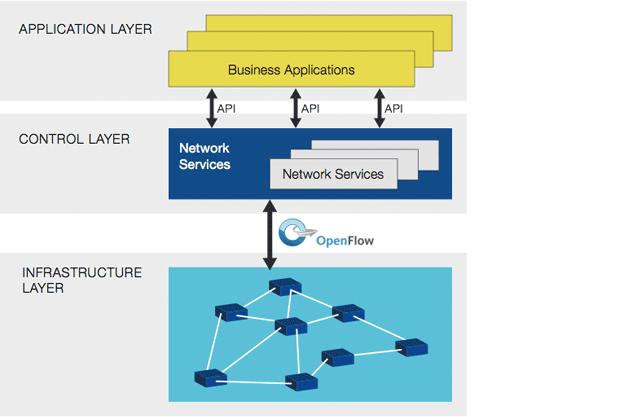
\includegraphics[width=20cm]{img/sdn-3layers.png}
   \caption{SDN 3 Layer Architecture}
   \label{fig:sdn3layer}
 \end{center}
 \end{figure}
\end{center}

SDN architecture is characterized by the following aspects:
\begin{itemize}
\item{\textbf{Open standards-based and vendor-neutral}}: Being implemented through open standards, SDN simplifies network design and operation. Instructions are provided by SDN controllers, which follow a particular set of open protocols and devices, instead of multiple, vendor-specific devices and protocols.
\item{\textbf{Directly programmable}}: Network control plane is directly programmable. This aspect is possible due to the fact that control planeis decoupled from forwarding plane.
\item{\textbf{Agile}}: Abstracting control from forwarding plane lets network administrators dynamically adjust network-wide traffic flow to meet particular needs of the network at each particular moment.
\item{\textbf{Centrally managed}}: Network intelligence is centralized in software-based SDN controllers. This kind of elements maintain a global view of the network topology. Network itself appears to applications and policy engines as a single, logical switch.
\item{\textbf{Programmatically configured}}: Network managers can configure, manage, secure, and optimize network resources through SDN very quickly via dynamic, automated SDN programs, which can be written themselves because the programs do not depend on proprietary software.
\end{itemize}

Previous detailed aspects make SDN technology to be one of the most recently boosting technologies, together with Cloud Computing and Big Data. Indeed, the increasing interests in all of them has also to do with the fact that all these technologies, together with Virtualization, are necessary linked between them.\\
\\
Next section shows how the market has increased in the last years, together with the big expectations that SDN tecnhology is supposed to have in the next years.

\subsection{SDN: Market share and expectations}

SDN is considered a boosting technology. In year 2013, the service-provider SDN market —hardware and software combined — was about \textbf{\$840 million in 2013} and is considered to grow to \textbf{\$15.6 billion in 2018}, according to a report released by ACG Research~\cite{SDN2018expectations00}.\\
\\
In this research, numbers don’t include the enterprise market, and apply only to service providers, including large-data-center owners such as Google and the big data centers of carriers such as NTT or AT\&T.\\
\\
Here’s how ACG’s 2018 forecast breaks down in the different main areas of SDN deployment: 

Data center:	\$3.3 billion
IP services:	\$4.2 billion
Metro networks:	\$4.3 billion
Core networks: \$3.8 billion
 
The numbers reflect only “live” SDN deployments, i.e.: cases where service providers would use the technology, and not just installing it for future use.

However, it must be remarked that expectations are even higher considering other reports. By mid 2013, market considered for year 2013 was about \$1.5 billion, and expectations for year 2018 was about \$35.5 billion according to a research by SDNCentral~\cite{SDN2018expectations01}.

\begin{center}
 \begin{figure}[htbp]
 \begin{center}
   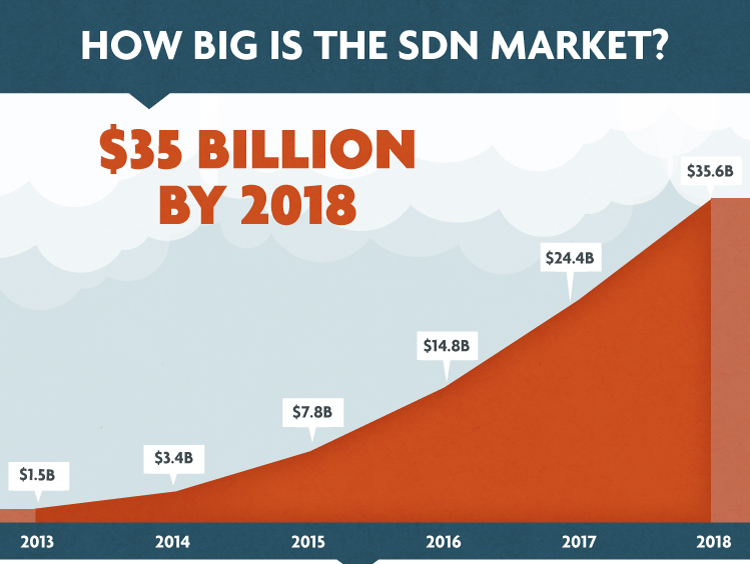
\includegraphics[width=20cm]{img/sdn_estimations_2018.png}
   \caption{SDN Market: 2018 SDNCentral estimations}
   \label{fig:sdn2018estimations}
 \end{center}
 \end{figure}
\end{center}

This last analysis and infographics doesn’t compare directly with previous one, as it wasn’t limited to service providers, and included SDN-ready equipment, sales that represent customers preparing for SDN even if they wouldn’t be using it immediately.\\
\\
Analyzing the data of this last report, a number of key takeaways must be highlighted:
\begin{enumerate}\itemsep0pt
 \item{The software-defined networking SDN market is expected to surpass \$35 billion in 2018}.
 \item{Adoption of SDN technology has accelerated in recent years from sales of \$10 million in 2007 to \$252 million in 2012}.
 \item{The emergence of the software-defined networking market is supported by growth in venture capital investment in SDN-focused companies}. Venture capital funding of SDN-related companies rose from \$10 million in 2007 to \$454 million in 2012.
\end{enumerate}

According to this report, the main three areas driving the rise in SDN are:
\begin{enumerate}\itemsep0pt
\item{Cloud Computing}
\item{Big Data}
\item{Mobility}
\end{enumerate}

Apart from pure SDN Market numbers, there are other aspects to consider. For example, the VC(Venture Capital) investment has grown, according to this report, from \$10 million in 2007 to \$454million in 2012.\\
\\
This report also considers that Networking Industry spending Percentage on SDN will rise from 2\% in 2013 to 40\% in 2014, with more than 220 companies by mid 2013, compared to the zero existing in 2009.\\
\\
Last, but not least, it must be remarked that up to more than \$1.5 billion has been invested in acquisitions of SDN related companies up to 2013, including the most remarkable one, the acquisition of Nicira Inc. by VMWare by July 2012, for approximately \$1.05 billion in cash plus approximately \$210 million of assumed unvested equity awards~\cite{VMWareAcquireNicira}.\\
\\
Far from giving a very detailed information on SDN market, this report has shown through all the numbers above how important is the SDN market and how important could be an OpenSource Software Project such as OpenDaylight, which is in the end a key component in SDN deployment.

\section{NVF}

Example for URL: more information here:
\url{http://developer.android.com/guide/topics/resources/localization.html}.

Example of table: In table~\ref{tab:i18nformats} you can find a list
of formats for localization~\cite{GPL}.

Example of \textbf{footnote}\footnote{\url{
http://translate.sourceforge.net/wiki/pootle/}, this is a footnote},
in ~\LaTeX~ suits nice.

Example of an in-document reference:
in section~\ref{chap:introduction} introductory concepts are explained.

\chapter{OpenDaylight: Technical Aspects}
\label{chap:odl_technical}

\chapter{OpenDaylight: Legal Aspects}
\label{chap:odl_legal}

\chapter{OpenDaylight: Economic Aspects}
\label{chap:odl_economic}

\chapter{OpenDaylight: Community Management}
\label{chap:odl_community}

\chapter{OpenDaylight: Project Evaluation}
\label{chap:odl_projeval}


%%%%%%%%%%%%%%%%%%%%%%%%%%%%%%%%%%%%%%

\chapter{Conclusions}
\label{chap:conclusions}

%%%%%%%%%%%%%%%%
% Review goals and objectives

\section{Evaluation}
%%%%%%%%%%%%%%%%%%%%%%%%%%%%%%%%%%%%%%

Review goals and objectives

%%%%%%%%%%%

\section{Lessons learned}
\label{sec:lessons}

\subsection{Lesson 1}
\begin{itemize}
 \item Explain here what anybody may learn from this document
\end{itemize}

\subsection{What I learned}
\begin{itemize}
 \item Explain what you learned writing this document
\end{itemize}

\subsection{Knowledge and skills acquired in the M.Sc. studies that helped me on
this work}
\begin{itemize}
 \item You can go subject by subject, explained in which aspects helped
you to do/write this project
 \item Or just mention only the main aspects/subjects

\end{itemize}

\section{Future work}
\label{sec:future}

\subsection{More on...}

If there is any aspect that is not fully covered, explain how it could be
better covered.

\subsection{Other aspects}

See the section about ``Scope'' and explain here other aspects that you didn't
cover but it could be nice to work on.


\subsection{Other focuses}

For example study similar projects, or apply other tools to do the same work.


%%%%%%%%%%%%%%%%%%%%%%%%%%%%%%%%%%%%%
\appendix

%%%%%%%%%%%%%%%%%%%%%%%%%%%%%%%%%%%%%%
\chapter{First Appendix}

\chapter{Second Appendix}

%%%%%%%%%%%%%%%%
% BIBLIOGRAPHY %
%%%%%%%%%%%%%%%%

\bibliographystyle{alpha}
\bibliography{bibliography}
\label{Bibliography}
\end{document}
